\documentclass[12pt]{article}

\usepackage[spanish, es-tabla, es-nodecimaldot]{babel}
\usepackage[utf8x]{inputenc}
\usepackage{amsmath}

\usepackage{hyperref}
\usepackage{url}
\usepackage{textcomp}
\usepackage{gensymb}
\usepackage[dvipsnames]{xcolor}

\usepackage{parskip}
\usepackage{fancyhdr}
\usepackage{multicol}
\usepackage{vmargin}
\usepackage{setspace}
\usepackage{geometry}

\usepackage{float}
\usepackage{array}
\usepackage{graphicx}
\graphicspath{{images/}}
\usepackage{wrapfig}
\usepackage{caption}
\usepackage{subcaption}

\setmarginsrb{2 cm}{1 cm}{2 cm}{1.5 cm}{0.5 cm}{1 cm}{1 cm}{1 cm} %{izq}{up}{der}{down}{Encabezado}
\title{Calor Especifico del Agua}
\author{Martín Alejandro Paredes Sosa}		

\makeatletter
\let\thetitle\@title
\let\theauthor\@author
\let\thedate\@date										
\makeatother

\pagestyle{fancy}
\fancyhf{}
%\rhead{Lic.. Física}
%\lhead{Informe 5: \thetitle}
\cfoot{\thepage}

\begin{document}
%====================================================================
\begin{center}
{ \large \bfseries \thetitle}
\end{center}
	\begin{minipage}{\textwidth}
		\begin{center} 
			\theauthor 
			\end{center}
	\end{minipage}
%===================================================================================================
	
\begin{abstract}
En esta experiencia se realizaron dos actividades cuyo principal objetivo fue determinar el calor específico del agua utilizando un calorímetro de resistencia eléctrica para calentar el agua mediante disipación.
\end{abstract}
\vspace{-1cm}
%===================================================================================================
\section{Introducción}
\vspace{-0.5cm}
Esta experiencia consistió en aumentar la temperatura de una masa de agua mediante la disipación de potencia eléctrica en calor, esto debido a que es muy dificil encontrar las propiedades calorimétricas de un calorímetro y de sus accesorios por separado pero usando la masa de agua que absorbe la misma cantidad de calor que el calorímetro se puede encontrar algo a lo que llamamos "equivalente en agua" la cual se considera una característica propia de cada calorímetro y sus accesorios.

Es de suma importancia encontrar este equivalente puesto que nos ayudará  a determinar el calor específico del agua.

El calor específico es la cantidad de calor que se necesita por unidad de masa para elevar la temperatura un grado Celsio. La relación entre calor y cambio de temperatura, se expresa normalmente en la forma que se muestra abajo, donde c es el calor específico.

\begin{equation}
Q = c m\Delta T
\end{equation}


se define la capacidad calorífica como la cantidad de calor que se debe suministrar a toda la masa de una sustancia para elevar su temperatura en una unidad (kelvin o grado Celsius).

La energía en forma de calor suministrado a un sistema de masa, con calor específico  y que cambio su temperatura en un intervalo$\Delta T$  está dada por la ecuación (1)
Por otra parte la energía en forma de calor disipada por la resistencia \textbf{R}, al pasar una corriente \textbf{I} a través de ella en un tiempo está dada por

\begin{equation}
Q = I^2 Rt = I V t
\end{equation}
Observando que la condición es que toda la energia eléctrica en forma de
trabajo es disipada en forma de calor por la resistencia. De tal manera
que si los lados izquierdos de estas ecuaciones son iguales se tiene que:
 
 
 \begin{equation}
 \Delta T = \frac{IV}{mc}t
 \end{equation}
 



\vspace{-0.5cm}
%===================================================================================================
\section{Desarrollo Experimental}
\vspace{-0.5cm}
La experiencia se dividió en dos actividades por lo tanto el desarrollo experimental se presenta en dos partes.

Para la primera actividad se usó un calorímetro, un agitador magnético, un termometro y una resistencia eléctrica.
\begin{itemize}
\item Se colocó una cantidad de agua fría en el calorímetro $T_{0f}$
\item Se midió la masa del calorímetro con agua $M_{f}$
\item Se esperó a que el agua fría llegara al equilibrio dentro del calorímetro.
\item Se agregó al calorímetro una masa de agua caliente a $T_{0c}$
\item Se midió la masa del calorímetro con agua $M_{c}$
\item Se esperó a que el interior del calorímetro alcanzara una $T_{fe}$ temperatura
de equilibrio.
\item Se obtuvó la masa equivalente en agua del calorímetro.
\end{itemize}

Para la segunda actividad se utilizó la masa equivalente encontrada en la actividad anterior y el mismo
material para encontrar el calor especifíco del agua.
\begin{itemize}
\item Se viritió aproximadamente 300 gr de agua en el calorímetro $m_{a}$
\item Se seleccionó una corriente de 1 A \item A tráves de un CAPSTONE se tomaron datos de la temperatura y el tiempo
\item Se conectaron dos multímetros a los calorímetros
\item Se midió la corriente y el voltaje en los multímetros y en la máquina de corriente.
\item Se tomarón lecturas cada 5 minutos durante 40 minutos.
\end{itemize}

%===================================================================================================

\section{Resultados}
Para la primera actividad se calculó la masa equivalente en agua del calorímetro a partir de la siguiente ecuación

\begin{equation}
M_{eq} = M_C \frac{T_{0c} - T_{fc} }{T_{fc} - T_{0f}} - M_f
\end{equation}

\begin{itemize}
\item $T_{0f} = 5.5 ^0 C$
\item $M_{f} = 155.62  g$
\item $M_{c} = 138.83 g$
\item $T_{0c} = 64.6 ^0 C$
\item $T_{fe} = 30.5 ^0 C$
\end{itemize}


Sustituyendo los datos anteriores en la ecuación (4) obtenemos:

$$M_{eq} = 33.7441 g$$

Para la segunda actividad se muestra una tabla con todas las mediciones.

\begin{table}[H]
\centering
\begin{tabular}{|c|c|c|c|c|}
\hline
V multímetro (V)& I multímetro (A) & V máquina (V) & I máquina (A)& Temperatura ($^0C$) \\ \hline
3.21& 1& 3.30 & 1.013& 14.4 \\ \hline
3.20& 1& 3.28 & 1.012& 15.3 \\ \hline
3.18& 1& 3.26 & 1.012& 16.1 \\ \hline
3.17& 1& 3.25 & 1.011& 16.8 \\ \hline
3.16& 1& 3.23 & 1.011& 17.5 \\ \hline
3.18& 1& 3.25 & 1.011& 18.3 \\ \hline
3.15& 1& 3.22 & 1.011& 18.9 \\ \hline
3.17& 1& 3.25 & 1.011& 19.6 \\ \hline
3.17& 1& 3.25 & 1.011& 20.3 \\ \hline

\end{tabular}
\caption{Mediciones}
\label{tab:traIso}
\end{table}



Se presenta la gráfica de temperatura vs tiempo.
\begin{figure}[H]
\begin{center}
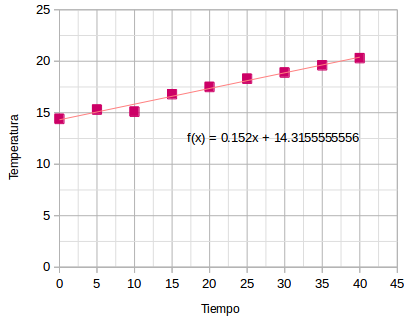
\includegraphics[width=0.7\textwidth]{pau.png}  
\caption{Amplificador con el Termopar}
\label{uno}
\end{center}
\end{figure}

Se realizó un ajuste lineal con los datos y se encontró que con el corte con el eje Ti $ 14.4 ^0C$ y la pendiente $0.152$ se puede aproximar el calor específico del agua

\begin{equation}
C_a = 0.625 \frac{J}{g ^0 C}
\end{equation}






%===================================================================================================
\section{Discusión}
Fue muy sorprendente que la masa equivalente en agua del calorímetro sea tan pequeña ya que se pensó que sería más grande debido a que las masas de agua y el calorímetro eran más grandes.
Analizando las gráficas podemos observar que la función corta el eje vertical en 14.4 grados.
Tuvimos un poco de confusión al consideran que valor del voltaje y de corriente tomar para calcular el calor específico del agua, pero al final se tomó como 1 A de corriente y 3.25 V de voltaje.
Creíamos que el valor del calor específico determinado sería muy diferente al que la literatura nos proporciona y efectivamente obtuvimos un resultado muy erróneo, esto debido a un mal manejo de datos y de la técnica usada para realizar esta experiencia.






%===================================================================================================
\section{Conclusiones}
El calor específico del agua determinado experimentalmente es de aproximadamente $0.066021 \frac{J}{g ^0 C}$
Comparado con el valor encontrado en la literatura de 4.181 $J/gK$ nos proporciona un valor de  casi el cien por ciento de error.
Dicho error se debe tanto a las incertidumbres de las herramientas de medición tanto a los errores humanos y tardanza al realizar el experimento, así como a los datos obtenidos del experimento.
Otro factor importante puede ser los valores de voltaje elegidos y las mediciones de las masas.
Por lo que podemos decir que no se logró el objetivo de esta experiencia.
%================================================================================================


\begin{thebibliography}{6}


\bibitem{acu}
Acuña, H. (2015). \textit{Manual de Guías de Experiencias en el Laboratorio de Termodinámica Clásica}.

\bibitem{W}
Zemansky, M., Dittman, R.(1990) \textit{Calor y Termodinámica}


\end{thebibliography}
%================================================================================================


\end{document}
